% =====================================================================
%  IEEE conference paper (IEEEtran)
%  Numbers in tables/*.tex and tables/macros.tex are regenerated from YOUR run:
%      python scripts/export_paper_tables.py
%  Compile: pdflatex main && bibtex main && pdflatex main && pdflatex main   (or upload paper/ to Overleaf)
% =====================================================================
\documentclass[conference]{IEEEtran}
\IEEEoverridecommandlockouts
\usepackage{cite}
\usepackage{amsmath,amssymb,amsfonts}
\usepackage{algorithm}
\usepackage{algpseudocode}
\usepackage{graphicx}
\usepackage{textcomp}
\usepackage{xcolor}
\usepackage{booktabs}
\usepackage{multirow}
\usepackage{tikz}
\usetikzlibrary{arrows.meta,positioning,fit,backgrounds}
\usepackage[hidelinks]{hyperref}

% AUTO-GENERATED by scripts/export_paper_tables.py
\newcommand{\NImages}{4591}
\newcommand{\NRef}{226}
\newcommand{\NAnom}{4365}
\newcommand{\NTest}{3099}
\newcommand{\NTestRef}{45}
\newcommand{\NTestAnom}{3054}
\newcommand{\NTrainRef}{90}
\newcommand{\CalN}{45}
\newcommand{\SelTopK}{0.001}
\newcommand{\SelLambda}{1}
\newcommand{\SelAlpha}{0.03}
\newcommand{\MinP}{0.0217}
\newcommand{\PoneThr}{9.72e-05}
\newcommand{\PoneAUC}{1.0000}
\newcommand{\PonePRAUC}{1.0000}
\newcommand{\PoneAcc}{0.9990}
\newcommand{\PoneBA}{0.9667}
\newcommand{\PoneFone}{0.9995}
\newcommand{\PonePrec}{0.9990}
\newcommand{\PoneRec}{1.0000}
\newcommand{\PoneSpec}{0.9333}
\newcommand{\PoneFPR}{0.0667}
\newcommand{\PoneFNR}{0.0000}
\newcommand{\PoneCost}{0.0010}
\newcommand{\PoneFP}{3}
\newcommand{\PoneFN}{0}
\newcommand{\PoneTP}{3054}
\newcommand{\PoneTN}{42}
\newcommand{\PoneDice}{0.4073}
\newcommand{\PoneIoU}{0.2643}
\newcommand{\PonePixAUC}{0.9205}
\newcommand{\PonePixAP}{0.4473}
\newcommand{\PtwoAUC}{1.0000}
\newcommand{\PtwoPRAUC}{1.0000}
\newcommand{\PtwoAcc}{0.9990}
\newcommand{\PtwoBA}{0.9667}
\newcommand{\PtwoFone}{0.9995}
\newcommand{\PtwoPrec}{0.9990}
\newcommand{\PtwoRec}{1.0000}
\newcommand{\PtwoSpec}{0.9333}
\newcommand{\PtwoFPR}{0.0667}
\newcommand{\PtwoFNR}{0.0000}
\newcommand{\PtwoCost}{0.0010}
\newcommand{\PtwoFP}{3}
\newcommand{\PtwoFN}{0}
\newcommand{\PtwoTP}{3054}
\newcommand{\PtwoTN}{42}
\newcommand{\PtwoDice}{0.5957}
\newcommand{\PtwoIoU}{0.4426}
\newcommand{\PtwoPixAUC}{0.9769}
\newcommand{\PtwoPixAP}{0.5491}
\newcommand{\DeltaDice}{0.1884}
\newcommand{\DeltaIoU}{0.1783}
\newcommand{\DeltaPixAUC}{0.0564}
\newcommand{\DeltaDiceRel}{46.2}
\newcommand{\DeltaIoURel}{67.5}
\newcommand{\PixGapRed}{70.9}

\newcommand{\Etil}{\tilde{E}}
\DeclareMathOperator*{\argmin}{arg\,min}
\DeclareMathOperator*{\argmax}{arg\,max}
\DeclareMathOperator{\med}{med}
\DeclareMathOperator{\MAD}{MAD}

\begin{document}

\title{Risk-Calibrated and Cost-Aware Anomaly Detection Visual Screening for Semiconductor Manufacturing Under Distribution Drift}

\author{
\IEEEauthorblockN{Varsha K}
\IEEEauthorblockA{\textit{M.Tech Data Science} \\
\textit{Rajalakshmi Engineering College}\\
Chennai, India \\
varsha.k.2025.mtechds@rajalakshmi.edu.in}
\and
\IEEEauthorblockN{Nalini Subramanian}
\IEEEauthorblockA{\textit{Department of Information Technology} \\
\textit{Rajalakshmi Engineering College}\\
Chennai, India}
}

\maketitle

% ---------------------------------------------------------------------
\begin{abstract}
Automated review of scanning electron microscope (SEM) images is required to keep pace with inspection volumes in semiconductor manufacturing, yet reconstruction-based anomaly detectors are usually deployed with an ad hoc threshold, without a quantified false-alarm risk, without regard for the asymmetric cost of a missed defect, and without evaluation under imaging drift. This paper presents RCC-ConvAE, a risk-calibrated and cost-aware decision framework built around a frozen two-dimensional convolutional autoencoder (ConvAE) that is trained exclusively on defect-free reference images. Global and localized top-$k$ reconstruction evidence are robustly normalized and fused, converted into split-conformal $p$-values using reference-only calibration images, and thresholded at a significance level selected by minimizing a $10{:}1$ false-negative to false-positive cost on a dedicated policy-validation set. The same error maps provide pixel-level defect masks. Evaluation is performed on the public Carinthia-S dataset (\NImages{} SEM images with expert masks) under a five-role, leakage-audited protocol in which the test partition is accessed only after every component has been frozen. The baseline and the proposed framework share the backbone and therefore obtain the same image-level ranking (ROC-AUC \PtwoAUC{}, balanced accuracy \PtwoBA{}, cost \PtwoCost{} per image), whereas RCC-ConvAE improves defect localization from a Dice score of \PoneDice{} to \PtwoDice{}, IoU from \PoneIoU{} to \PtwoIoU{}, and pixel AUROC from \PonePixAUC{} to \PtwoPixAUC{}. A nine-condition photometric and blur drift study quantifies the benefit of label-free recalibration.
\end{abstract}

\begin{IEEEkeywords}
anomaly detection, convolutional autoencoder, conformal prediction, cost-sensitive decision, defect localization, distribution shift, scanning electron microscopy, semiconductor manufacturing
\end{IEEEkeywords}

% =====================================================================
\section{Introduction and Literature Review}
% =====================================================================
Yield in semiconductor manufacturing is governed by the ability to detect and localize defects early, before a faulty layer propagates through subsequent process steps. Scanning electron microscopy (SEM) provides nanometer-scale visibility of wafer surfaces, but the volume of review images produced by modern fabs exceeds what process engineers can inspect manually. Automated visual screening is therefore required; however, three properties of the domain complicate the use of conventional supervised learning. First, defect appearance is open-ended: new mechanisms emerge whenever a recipe, tool, or material changes, so a closed-set classifier trained on historical defect types is inherently incomplete. Second, the consequences of errors are asymmetric: a missed defect can lead to scrapped lots or field failures, whereas a false alarm costs only an additional review. Third, imaging conditions drift over time because of beam current, detector gain, focus, and charging effects, and a screening threshold tuned on yesterday's images may no longer be valid today.

Unsupervised anomaly detection addresses the first issue by modelling only the appearance of normal, or \emph{reference}, samples. Autoencoders learn a compressed representation of reference data and flag inputs that cannot be reconstructed faithfully~\cite{hinton2006,masci2011}. In the semiconductor domain, Gorman \emph{et al.}~\cite{gorman2023} showed that one-dimensional convolutional autoencoders applied to batch-process sensor traces, combined with \emph{localized} rather than global reconstruction errors, detect anomalous batches with a reported AUC of 1.00. For images, Bergmann \emph{et al.} introduced the MVTec~AD benchmark~\cite{bergmann2019mvtec} and demonstrated that structural rather than pixel-wise reconstruction losses improve defect segmentation~\cite{bergmann2019ssim}. Feature-embedding methods such as PaDiM~\cite{defard2021} and PatchCore~\cite{roth2022} subsequently advanced the state of the art on natural-image benchmarks, and recent surveys summarize the broader deep anomaly detection landscape~\cite{pang2021}. On SEM data specifically, Barusco \emph{et al.}~\cite{barusco2025} benchmarked nine visual anomaly detection methods and observed that the domain gap between photographs and microscopy materially alters method rankings. Supervised convolutional networks have been widely used for wafer-map pattern classification~\cite{nakazawa2018}, but they require exhaustive defect labels.

The second and third issues concern the \emph{decision} rather than the \emph{score}. Conformal prediction~\cite{vovk2005,angelopoulos2021} provides distribution-free, finite-sample guarantees, and conformal $p$-values for outlier detection control the false-alarm rate using only inlier calibration data~\cite{bates2023,laxhammar2015}. Cost-sensitive learning theory establishes that the optimal operating point depends on the ratio of misclassification costs~\cite{elkan2001}. Robustness to corruptions and dataset shift has been studied systematically for image classifiers~\cite{hendrycks2019,rabanser2019}, and miscalibration of deep networks under such conditions is well documented~\cite{guo2017}. These strands have rarely been combined for reference-only SEM screening with pixel-level ground truth.

This paper integrates them into a single, auditable framework. The contributions are as follows:
\begin{itemize}
\item A reference-only two-dimensional ConvAE baseline for SEM screening, adapted from the localized reconstruction-error principle of~\cite{gorman2023}.
\item RCC-ConvAE, which fuses robustly normalized global and local top-$k$ evidence, converts it to conformal $p$-values using reference-only calibration images, and selects the significance level by minimizing manufacturing cost.
\item Pixel-level localization evaluated against expert masks using Dice, IoU, and pixel AUROC.
\item A drift study with nine imaging conditions that compares frozen policies with label-free recalibration.
\item A five-role data protocol with an automated leakage audit that ensures the test set never influences any design choice.
\end{itemize}

% =====================================================================
\section{Proposal and Existing System Analysis}
% =====================================================================
The existing approach considered as the baseline is the convolutional autoencoder with localized reconstruction error of Gorman \emph{et al.}~\cite{gorman2023}, together with its direct two-dimensional adaptation for images.

\subsection{System}
The existing system operates on multivariate time-series sensor data acquired during batch manufacturing, in which each batch is represented by a fixed-length sequence of process-variable readings. A one-dimensional convolutional autoencoder is trained on batches that are considered normal. The deployment environment is offline batch-level quality assessment, where each completed batch is scored once and compared with a threshold.

\subsection{Method}
The encoder applies one-dimensional convolutions along the time axis to compress each batch into a latent representation, and the decoder reconstructs the original sequence. Instead of summarizing the reconstruction error of the whole sequence by a single mean value, the method computes errors over localized temporal windows and uses the most anomalous local region as the batch score. This design prevents a short but severe deviation from being diluted by a long, normal remainder of the batch. The anomaly score is then compared against a threshold derived from the distribution of errors on normal data.

\subsection{Result Abstract}
On the evaluated batch-process data, the localized reconstruction-error score separated anomalous from normal batches perfectly, with a reported area under the ROC curve of 1.00~\cite{gorman2023}. The result establishes that localized reconstruction evidence is more discriminative than a global average error for manufacturing anomalies in which the abnormal signature is spatially or temporally confined.

\subsection{Limitations and Drawbacks}
Although effective for its intended setting, the existing approach leaves several gaps that motivate the proposed system:
\begin{enumerate}
\item \emph{Modality.} The method is designed for one-dimensional sensor traces and does not address two-dimensional SEM images, in which defects are spatially localized and surrounded by textured, repetitive structure.
\item \emph{Uncalibrated threshold.} AUC measures ranking quality only. The operating threshold is not accompanied by a finite-sample guarantee on the false-alarm rate, so the risk of each decision is unquantified.
\item \emph{Cost blindness.} The threshold does not reflect the asymmetric cost of a missed defect versus a false alarm, and therefore does not minimize the expected loss of a production line.
\item \emph{No pixel-level output.} The method identifies anomalous batches, but for visual inspection an engineer also needs to know \emph{where} the defect lies. A direct 2-D adaptation that uses the raw error map produces noisy, speckled masks.
\item \emph{Static deployment.} Robustness to changing acquisition conditions is not evaluated, and no procedure is provided to recalibrate the decision rule when the input distribution shifts.
\item \emph{Saturated metric.} A reported AUC of 1.00 cannot be improved upon; further progress must therefore be measured by decision quality, calibration, localization, and robustness rather than by ranking accuracy alone.
\end{enumerate}
The proposed RCC-ConvAE retains the core insight of localized reconstruction evidence while adding the decision, localization, and drift layers that the existing system lacks.

% =====================================================================
\section{System Design and Architecture}
% =====================================================================
Fig.~\ref{fig:arch} summarizes the pipeline, which follows an Input $\rightarrow$ Modules $\rightarrow$ Output flow.

\begin{figure*}[t]
\centering
\resizebox{\textwidth}{!}{%
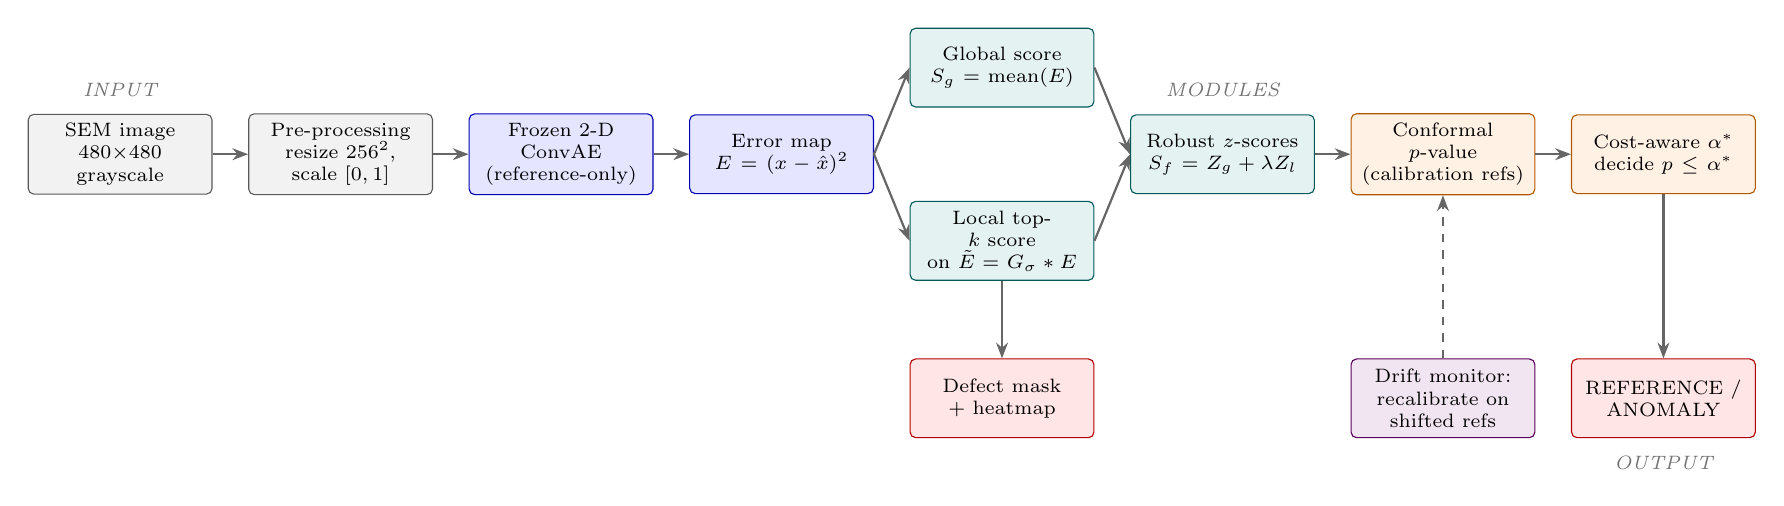
\begin{tikzpicture}[
  box/.style={draw=#1!70!black, fill=#1!10, rounded corners=2pt, align=center, font=\scriptsize, minimum height=10mm, text width=21mm},
  box/.default=blue,
  arr/.style={-{Stealth[length=2mm]}, thick, draw=black!60}]
\node[box=gray]   (in)   at (0,0)      {SEM image\\$480{\times}480$ grayscale};
\node[box=gray]   (pre)  at (2.8,0)    {Pre-processing\\resize $256^2$, scale $[0,1]$};
\node[box=blue]   (ae)   at (5.6,0)    {Frozen 2-D ConvAE\\(reference-only)};
\node[box=blue]   (em)   at (8.4,0)    {Error map\\$E=(x-\hat x)^2$};
\node[box=teal]   (g)    at (11.2,1.1) {Global score\\$S_g=\operatorname{mean}(E)$};
\node[box=teal]   (l)    at (11.2,-1.1){Local top-$k$ score\\on $\tilde E=G_\sigma * E$};
\node[box=teal]   (fu)   at (14.0,0)   {Robust $z$-scores\\$S_f=Z_g+\lambda Z_l$};
\node[box=orange] (cp)   at (16.8,0)   {Conformal $p$-value\\(calibration refs)};
\node[box=orange] (dec)  at (19.6,0)   {Cost-aware $\alpha^*$\\decide $p\le\alpha^*$};
\node[box=red]    (mask) at (11.2,-3.1){Defect mask\\+ heatmap};
\node[box=violet] (drift) at (16.8,-3.1){Drift monitor:\\recalibrate on shifted refs};
\node[box=red]    (out)  at (19.6,-3.1){REFERENCE /\\ANOMALY};
\draw[arr] (in)--(pre); \draw[arr] (pre)--(ae); \draw[arr] (ae)--(em);
\draw[arr] (em.east)--(g.west); \draw[arr] (em.east)--(l.west);
\draw[arr] (g.east)--(fu.west); \draw[arr] (l.east)--(fu.west);
\draw[arr] (fu)--(cp); \draw[arr] (cp)--(dec); \draw[arr] (dec)--(out);
\draw[arr] (l)--(mask);
\draw[arr, dashed] (drift)--(cp);
\node[font=\scriptsize\itshape, text=black!55, above=1mm of in] {INPUT};
\node[font=\scriptsize\itshape, text=black!55, above=1mm of fu] {MODULES};
\node[font=\scriptsize\itshape, text=black!55, below=1mm of out] {OUTPUT};
\end{tikzpicture}}
\caption{Architecture of the proposed RCC-ConvAE screening pipeline. Phase~1 uses only the upper path up to the global score and a calibration-quantile threshold; Phase~2 adds local evidence, fusion, conformal calibration, cost-aware decision, localization, and drift recalibration on the same frozen backbone.}
\label{fig:arch}
\end{figure*}

\subsection{Input Layer}
The input is a single grayscale SEM image of an unstructured wafer surface. Images are resized from $480\times480$ to $256\times256$ pixels by bilinear interpolation and scaled to $[0,1]$. During training and calibration, the accompanying expert mask is used only to derive the image label (empty mask $\Rightarrow$ reference, non-empty mask $\Rightarrow$ anomaly) and the pixel-level ground truth for evaluation; the metadata class identifier is never used as the normality label.

\subsection{Reconstruction Module}
A convolutional autoencoder trained exclusively on reference images reconstructs the input. Because the network has only seen defect-free surface texture, it reproduces the repetitive background faithfully while failing to reproduce foreign structures such as particles, scratches, or residues. After training, the weights are frozen and cryptographically hashed so that all later modules operate on an identical backbone.

\subsection{Evidence Module}
The squared difference between the input and its reconstruction yields a per-pixel error map. Two complementary statistics are extracted: a global score, which averages the error over the whole image and captures diffuse abnormality, and a local score, which averages only the top-$k$ fraction of a Gaussian-smoothed error map and captures small but intense defects that would otherwise be diluted.

\subsection{Normalization and Fusion Module}
Because the global and local statistics differ in scale, each is converted to a robust $z$-score using the median and median absolute deviation of validation reference images. The two $z$-scores are fused linearly with a weight $\lambda$ chosen on validation data.

\subsection{Risk-Calibration Module}
The fused score of a new image is compared with the fused scores of a held-out set of calibration reference images to obtain a conformal $p$-value, which expresses how atypical the image is relative to the reference population, with a finite-sample guarantee on the reference false-alarm rate.

\subsection{Cost-Aware Decision Module}
The image is labelled ANOMALY when its $p$-value does not exceed a significance level $\alpha^*$. The level $\alpha^*$ is chosen on a policy-validation set so that the total cost $10\cdot\mathrm{FN}+1\cdot\mathrm{FP}$ is minimized.

\subsection{Localization Module}
The smoothed error map is thresholded at a quantile of validation reference pixel errors, and a morphological opening removes isolated false-positive pixels. The threshold quantile and opening radius are selected to maximize mean Dice on validation anomalies.

\subsection{Output Layer and Drift Monitor}
For each image the system outputs the REFERENCE/ANOMALY decision, the global, local, and fused scores, the $p$-value and the active $\alpha^*$, a heatmap, and a binary defect mask. When the acquisition conditions change, the drift monitor re-scores a small set of reference images acquired under the new conditions and replaces the calibration scores, without retraining and without any defect labels.

% =====================================================================
\section{Algorithm Design and Mathematical Programming}
% =====================================================================
\subsection{Problem Definition}
Let $\mathcal{D}=\{(x_j,m_j)\}_{j=1}^{M}$ denote SEM images $x_j\in[0,1]^{H\times W}$ with binary masks $m_j\in\{0,1\}^{H\times W}$. The image label is defined by the mask,
\begin{equation}
y_j=\mathbb{1}\!\left[\textstyle\sum_{u} m_{j,u}>0\right],
\end{equation}
so that $y_j=0$ denotes a reference image and $y_j=1$ an anomaly. $\mathcal{D}$ is partitioned into disjoint roles $\mathcal{D}_{\mathrm{tr}},\mathcal{D}_{\mathrm{val}},\mathcal{D}_{\mathrm{cal}},\mathcal{D}_{\mathrm{pol}},\mathcal{D}_{\mathrm{te}}$, where $\mathcal{D}_{\mathrm{tr}}$ and $\mathcal{D}_{\mathrm{cal}}$ contain only reference images. The goal is a decision rule $\delta:[0,1]^{H\times W}\to\{0,1\}$ and a mask predictor $\hat m$ whose parameters depend on $\mathcal{D}\setminus\mathcal{D}_{\mathrm{te}}$ only.

\subsection{Reference-Only Convolutional Autoencoder}
The autoencoder $f_\theta=g_\phi\circ h_\psi$ consists of an encoder $h_\psi$ with four strided convolutions (kernel 4, stride 2) followed by ReLU activations, mapping $256\times256\times1$ to a $16\times16\times64$ latent tensor, and a mirrored decoder $g_\phi$ of four transposed convolutions ending in a sigmoid. The parameters solve
\begin{equation}
\theta^*=\argmin_{\theta}\;\frac{1}{|\mathcal{D}_{\mathrm{tr}}|}\sum_{x\in\mathcal{D}_{\mathrm{tr}}}\frac{1}{N}\big\lVert \mathcal{A}(x)-f_\theta(\mathcal{A}(x))\big\rVert_2^2,
\end{equation}
where $N=HW$ and $\mathcal{A}$ is a random flip/rotation augmentation. Training uses Adam~\cite{kingma2015} and stops early when the reconstruction loss on the validation reference images has not improved for 20 epochs.

\subsection{Evidence Extraction}
For an image $x$ with reconstruction $\hat x=f_{\theta^*}(x)$,
\begin{align}
E_u &= (x_u-\hat x_u)^2, \qquad \Etil = G_\sigma * E,\\
S_g(x) &= \frac{1}{N}\sum_{u=1}^{N} E_u,\\
S_l^{(k)}(x) &= \frac{1}{K}\sum_{u\in\mathcal{T}_K(\Etil)}\Etil_u,\qquad K=\lceil kN\rceil,
\end{align}
where $G_\sigma$ is a Gaussian kernel with $\sigma=2$ pixels and $\mathcal{T}_K(\cdot)$ returns the indices of the $K$ largest entries. Phase~1 declares an anomaly when $S_g(x)\ge\tau_{0.95}$, the finite-sample corrected 95th percentile of $\{S_g(x):x\in\mathcal{D}_{\mathrm{cal}}\}$.

\subsection{Robust Normalization and Fusion}
With statistics fitted on the reference images of $\mathcal{D}_{\mathrm{val}}$,
\begin{equation}
Z_\bullet(x)=\frac{S_\bullet(x)-\med(S_\bullet)}{1.4826\,\MAD(S_\bullet)},\quad
S_f(x)=Z_g(x)+\lambda\,Z_l^{(k)}(x).
\end{equation}
The pair $(k,\lambda)$ is chosen from $\mathcal{K}=\{0.001,0.005,0.01,0.02,0.05\}$ and $\Lambda=\{0,0.25,\dots,3\}$ by
\begin{equation}
(k^*,\lambda^*)=\argmax_{k\in\mathcal{K},\,\lambda\in\Lambda}\;\mathrm{AUC}_{\mathcal{D}_{\mathrm{val}}}\!\big(S_f\big),
\end{equation}
with ties broken by PR-AUC, then by the equal-weight prior $|\lambda-1|$, then by smaller $k$.

\subsection{Conformal Risk Calibration}
Let $\{s_i\}_{i=1}^{n}=\{S_f(x):x\in\mathcal{D}_{\mathrm{cal}}\}$. The conformal $p$-value of a new image is
\begin{equation}
p(x)=\frac{1+\#\{i: s_i\ge S_f(x)\}}{n+1}.
\end{equation}
If a new reference image is exchangeable with $\mathcal{D}_{\mathrm{cal}}$, then $\Pr[p(x)\le\alpha]\le\alpha$ for every $\alpha\in(0,1)$~\cite{vovk2005,bates2023}; hence $\alpha$ upper-bounds the false-alarm rate on reference images. The smallest attainable $p$-value is $1/(n+1)$, which equals \MinP{} for $n=\CalN{}$.

\subsection{Cost-Aware Operating Point}
With costs $C_{\mathrm{FN}}=10$ and $C_{\mathrm{FP}}=1$, the significance level is the solution of the integer program
\begin{equation}
\alpha^*=\argmin_{\alpha\in\mathcal{G}}\; C_{\mathrm{FN}}\,\mathrm{FN}(\alpha)+C_{\mathrm{FP}}\,\mathrm{FP}(\alpha),
\end{equation}
where $\mathrm{FN}(\alpha)=\sum_{x\in\mathcal{D}_{\mathrm{pol}}} y\,\mathbb{1}[p(x)>\alpha]$ and $\mathrm{FP}(\alpha)=\sum_{x\in\mathcal{D}_{\mathrm{pol}}}(1-y)\,\mathbb{1}[p(x)\le\alpha]$, optionally subject to a yield constraint $|\mathcal{D}_{\mathrm{pol}}|^{-1}\sum\mathbb{1}[p(x)\le\alpha]\le\rho$, over a grid $\mathcal{G}\subset[0.01,0.30]$, choosing the smallest $\alpha$ among ties. The final rule is $\delta(x)=\mathbb{1}[p(x)\le\alpha^*]$.

\subsection{Pixel-Level Localization}
The predicted mask is
\begin{equation}
\hat m(x)=\mathcal{O}_r\!\left(\mathbb{1}\big[\Etil(x)\ge\tau_q\big]\right),
\end{equation}
where $\tau_q$ is the $q$-quantile of smoothed pixel errors of validation reference images and $\mathcal{O}_r$ is a binary opening with a disk of radius $r$. The pair $(q^*,r^*)$ maximizes the mean Dice coefficient $2|\hat m\cap m|/(|\hat m|+|m|)$ over the anomalies of $\mathcal{D}_{\mathrm{val}}$.

\subsection{Drift and Recalibration}
A drift condition is an image operator $T_c$ (brightness offset, contrast scaling, gamma, additive Gaussian noise, or Gaussian blur). Under a \emph{frozen} policy, $T_c$ is applied to test images only. Under \emph{recalibration}, the calibration scores are recomputed as $\{S_f(T_c(x)):x\in\mathcal{D}_{\mathrm{cal}}\}$, while $\theta^*$, $k^*$, $\lambda^*$, the normalization statistics, and $\alpha^*$ remain fixed. Recalibration requires only reference images and no labels. Because recalibration changes only the threshold and not the score, the ROC-AUC of a frozen and a recalibrated policy is identical by construction; the effect appears in FPR, FNR, balanced accuracy, and cost.

Algorithms~\ref{alg:fit} and~\ref{alg:infer} give the fitting and inference procedures.

\begin{algorithm}[t]
\caption{RCC-ConvAE policy fitting (test data never accessed)}
\label{alg:fit}
\footnotesize
\begin{algorithmic}[1]
\Require $\mathcal{D}_{\mathrm{tr}},\mathcal{D}_{\mathrm{val}},\mathcal{D}_{\mathrm{cal}},\mathcal{D}_{\mathrm{pol}}$; grids $\mathcal{K},\Lambda,\mathcal{G}$; costs $C_{\mathrm{FN}},C_{\mathrm{FP}}$
\Ensure frozen policy $\Pi=(\theta^*,\mathrm{stats},k^*,\lambda^*,\{s_i\},\alpha^*,\tau_{q^*},r^*)$
\State Train $f_\theta$ on $\mathcal{D}_{\mathrm{tr}}$ (references) with Adam; early-stop on references of $\mathcal{D}_{\mathrm{val}}$; freeze $\theta^*$
\ForAll{$x\in\mathcal{D}_{\mathrm{val}}\cup\mathcal{D}_{\mathrm{cal}}\cup\mathcal{D}_{\mathrm{pol}}$}
  \State $E\gets(x-f_{\theta^*}(x))^2$;\; $\Etil\gets G_\sigma*E$
  \State $S_g(x)\gets\mathrm{mean}(E)$;\; $S_l^{(k)}(x)\gets\mathrm{mean}(\mathrm{top}_k(\Etil))\ \forall k\in\mathcal{K}$
\EndFor
\State $\mathrm{stats}\gets(\med,\MAD)$ of $S_g,S_l^{(k)}$ on references of $\mathcal{D}_{\mathrm{val}}$
\State $(k^*,\lambda^*)\gets\argmax_{k,\lambda}\mathrm{AUC}_{\mathcal{D}_{\mathrm{val}}}(Z_g+\lambda Z_l^{(k)})$
\State $\{s_i\}\gets\{S_f(x):x\in\mathcal{D}_{\mathrm{cal}}\}$
\For{$\alpha\in\mathcal{G}$}
  \State $\hat y(x)\gets\mathbb{1}[p(x)\le\alpha]$ for $x\in\mathcal{D}_{\mathrm{pol}}$
  \State $\mathrm{Cost}(\alpha)\gets C_{\mathrm{FN}}\cdot\mathrm{FN}+C_{\mathrm{FP}}\cdot\mathrm{FP}$
\EndFor
\State $\alpha^*\gets$ smallest $\arg\min_\alpha\mathrm{Cost}(\alpha)$
\State $(q^*,r^*)\gets\argmax_{q,r}\overline{\mathrm{Dice}}$ on anomalies of $\mathcal{D}_{\mathrm{val}}$
\State \Return $\Pi$ \Comment{hash and freeze before evaluating $\mathcal{D}_{\mathrm{te}}$}
\end{algorithmic}
\end{algorithm}

\begin{algorithm}[t]
\caption{RCC-ConvAE screening of a new SEM image}
\label{alg:infer}
\footnotesize
\begin{algorithmic}[1]
\Require image $x$, frozen policy $\Pi$
\State $x\gets\mathrm{resize}(x,256)/255$;\; $\hat x\gets f_{\theta^*}(x)$
\State $E\gets(x-\hat x)^2$;\; $\Etil\gets G_\sigma*E$
\State $Z_g\gets(\mathrm{mean}(E)-\med_g)/(1.4826\,\MAD_g)$
\State $Z_l\gets(\mathrm{mean}(\mathrm{top}_{k^*}(\Etil))-\med_l)/(1.4826\,\MAD_l)$
\State $S_f\gets Z_g+\lambda^* Z_l$;\; $p\gets\big(1+\#\{s_i\ge S_f\}\big)/(n+1)$
\State $\mathrm{decision}\gets$ \textsc{Anomaly} \textbf{if} $p\le\alpha^*$ \textbf{else} \textsc{Reference}
\State $\hat m\gets\mathcal{O}_{r^*}(\mathbb{1}[\Etil\ge\tau_{q^*}])$
\State \Return $\mathrm{decision},\,p,\,S_f,\,\Etil,\,\hat m$
\end{algorithmic}
\end{algorithm}

The per-image cost of inference is one forward pass of the autoencoder plus $O(N)$ operations for smoothing, partial sorting, and thresholding; calibration adds an $O(\log n)$ binary search.

% =====================================================================
\section{Implementation}
% =====================================================================
\subsection{Dataset}
Carinthia-S~\cite{carinthia2025} contains \NImages{} SEM images of a single production layer of unstructured semiconductor wafers, each $480\times480$ pixels in grayscale, with an expert-validated binary segmentation mask and a six-valued metadata class. Automated verification of the files found \NRef{} empty masks (reference) and \NAnom{} non-empty masks (anomaly), no missing files, no duplicate names, and consistent image--mask dimensions. Because reference images are scarce (4.9\,\%), they are divided across all five roles, whereas anomalies, stratified by metadata class, are assigned only to validation, policy-validation, and test roles (Table~\ref{tab:split}).

\begin{table}[t]
\centering
\caption{Leakage-free five-role split (seed 42)}
\label{tab:split}
% AUTO-GENERATED
\begin{tabular}{lccc}
\toprule
Role & Reference & Anomaly & Total \\
\midrule
Train & 90 & 0 & 90 \\
Validation & 23 & 437 & 460 \\
Calibration & 45 & 0 & 45 \\
Policy Validation & 23 & 874 & 897 \\
Test & 45 & 3054 & 3099 \\
\bottomrule
\end{tabular}

\end{table}

\subsection{Leakage Control}
All pairwise intersections between the test set and the other roles are verified to be empty, the training and calibration roles are verified to contain only references, and the checkpoint and policies are hashed before the single test evaluation. An automated test additionally multiplies every test score by $10^3$ and confirms that no fitted parameter changes.

\subsection{Environment and Hyper-Parameters}
The system was implemented in Python~3.11 with PyTorch~\cite{paszke2019} for the autoencoder, scikit-learn and SciPy for metrics and morphology, Matplotlib and Plotly for figures, and Streamlit for the interactive dashboard. Experiments were run on a CPU-only Windows~11 laptop, demonstrating that the framework does not require a GPU. The autoencoder has 591{,}361 parameters (base width 32, latent 64 channels). Training used a batch size of 8, a learning rate of $10^{-3}$, weight decay of $10^{-5}$, at most 150 epochs, and patience 20. The global seed was fixed to 42. The localization search grid comprised quantiles $\{0.95,\dots,0.9995\}$ and opening radii $\{0,1,2\}$, and pixel AUROC and average precision were estimated with a 10{,}000-bin streaming histogram to bound memory.

\subsection{Software Artefacts}
A single command reproduces the ten pipeline stages (verification, training, Phase-1 calibration and evaluation, freezing, Phase-2 fitting, final evaluation, ablation, drift, reporting, and packaging checks). The dashboard provides single-image and batch screening with CSV export, together with interactive views of all metrics, the ablation, and the drift study.

% =====================================================================
\section{Results and Discussion}
% =====================================================================
All results are reported on the held-out test set (\NTest{} images: \NTestRef{} references and \NTestAnom{} anomalies) after every component was frozen. The validation-selected hyper-parameters were $k^*=\SelTopK{}$, $\lambda^*=\SelLambda{}$, and $\alpha^*=\SelAlpha{}$.

\begin{table}[t]
\centering
\caption{Image- and pixel-level results on the test set}
\label{tab:main}
% AUTO-GENERATED
\begin{tabular}{lcc}
\toprule
Metric & Phase~1 ConvAE & RCC-ConvAE \\
\midrule
ROC-AUC & 1.0000 & 1.0000 \\
PR-AUC & 1.0000 & 1.0000 \\
Accuracy & 0.9990 & 0.9990 \\
Balanced accuracy & 0.9667 & 0.9667 \\
Precision & 0.9990 & 0.9990 \\
Recall & 1.0000 & 1.0000 \\
Specificity & 0.9333 & 0.9333 \\
F1-score & 0.9995 & 0.9995 \\
FPR & 0.0667 & 0.0667 \\
FNR & 0.0000 & 0.0000 \\
Cost / image & 0.0010 & 0.0010 \\
\midrule
TN / FP & 42 / 3 & 42 / 3 \\
FN / TP & 0 / 3054 & 0 / 3054 \\
\midrule
Dice & 0.4073 & 0.5957 \\
IoU & 0.2643 & 0.4426 \\
Pixel AUROC & 0.9205 & 0.9769 \\
Pixel AP & 0.4473 & 0.5491 \\
\bottomrule
\end{tabular}

\end{table}

\subsection{Image-Level Screening}
Table~\ref{tab:main} shows that the reference-only ConvAE separates anomalous from reference images almost perfectly, with a ROC-AUC of \PoneAUC{} and PR-AUC of \PonePRAUC{}. The Phase-1 and RCC-ConvAE policies produce the same image-level metrics (balanced accuracy \PtwoBA{}, FPR \PtwoFPR{}, FNR \PtwoFNR{}). This parity is expected and is reported as observed: both policies rely on the same frozen backbone, and at this level of separability the calibration-quantile threshold and the cost-optimal conformal threshold fall into the same gap between the two score populations. The practical difference is that the RCC-ConvAE decision carries a calibrated interpretation, namely that at most a fraction $\alpha^*$ of reference images is expected to be flagged, and that $\alpha^*$ was selected to minimize the operational cost of \PtwoCost{} per image rather than fixed arbitrarily.

Because the test set contains approximately 98.5\,\% anomalies, accuracy, F1, and PR-AUC are dominated by the anomaly class. Balanced accuracy, FPR, and cost per image are therefore the more informative image-level indicators. The FPR of \PtwoFPR{} corresponds to \PtwoFP{} false alarm(s) among the \NTestRef{} test references, which is consistent with the conformal guarantee at the selected $\alpha^*$.

\subsection{Pixel-Level Localization}
The principal quantitative gain of RCC-ConvAE lies in localization. Relative to the raw-map baseline, the Dice coefficient rises from \PoneDice{} to \PtwoDice{} (a relative improvement of \DeltaDiceRel\,\%), IoU rises from \PoneIoU{} to \PtwoIoU{} (\DeltaIoURel\,\%), and pixel AUROC rises from \PonePixAUC{} to \PtwoPixAUC{}. The raw squared-error map responds to high-frequency texture and edge misalignment across the whole image, producing many isolated false-positive pixels. Gaussian smoothing integrates evidence over a neighbourhood, so that coherent defect regions are reinforced while scattered texture residuals are suppressed, and the validation-selected opening removes the remaining speckle. The same smoothed map supplies the local top-$k$ evidence, so that image-level and pixel-level outputs are derived from a consistent representation.

\IfFileExists{figures/localization_examples.png}{
\begin{figure}[t]
\centering
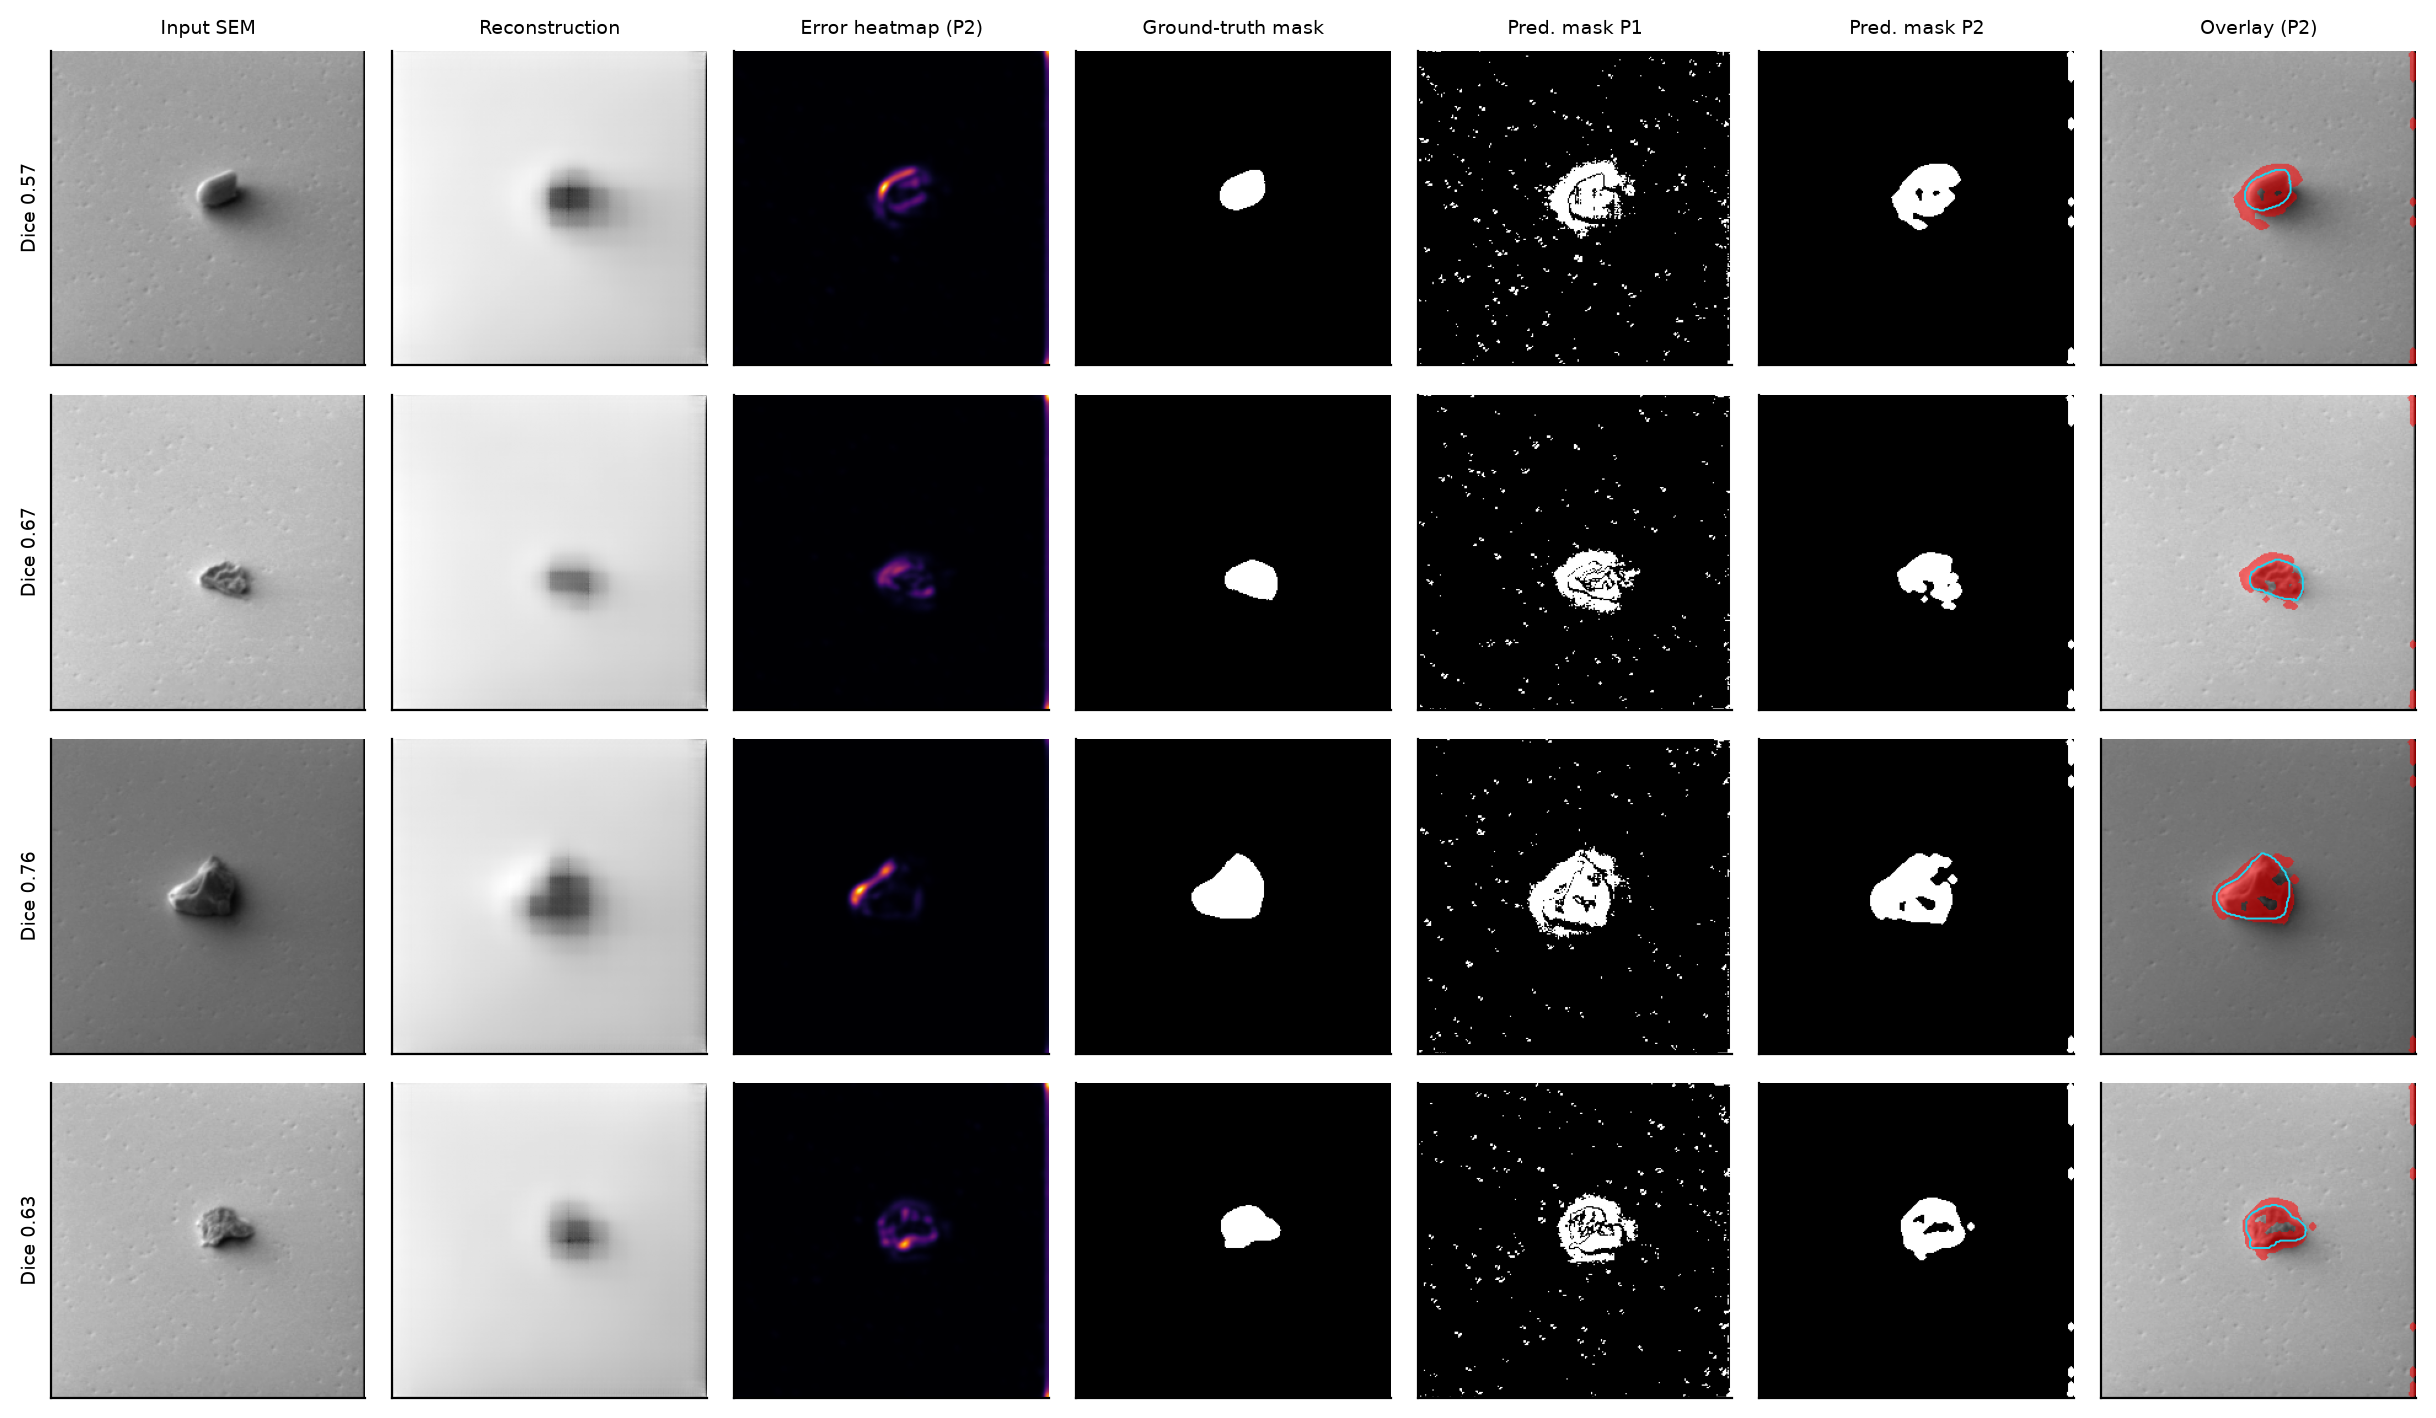
\includegraphics[width=\columnwidth]{figures/localization_examples.png}
\caption{Test examples: input, reconstruction, smoothed error heatmap, ground-truth mask, Phase-1 and RCC-ConvAE masks, and overlay.}
\label{fig:loc}
\end{figure}}{}

\IfFileExists{figures/roc_curve.png}{
\begin{figure}[t]
\centering
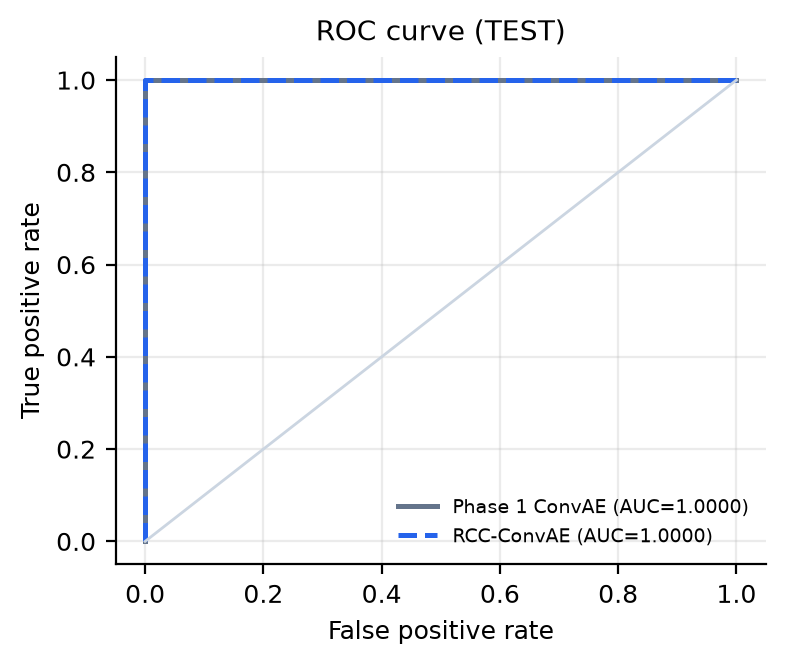
\includegraphics[width=0.49\columnwidth]{figures/roc_curve.png}\hfill
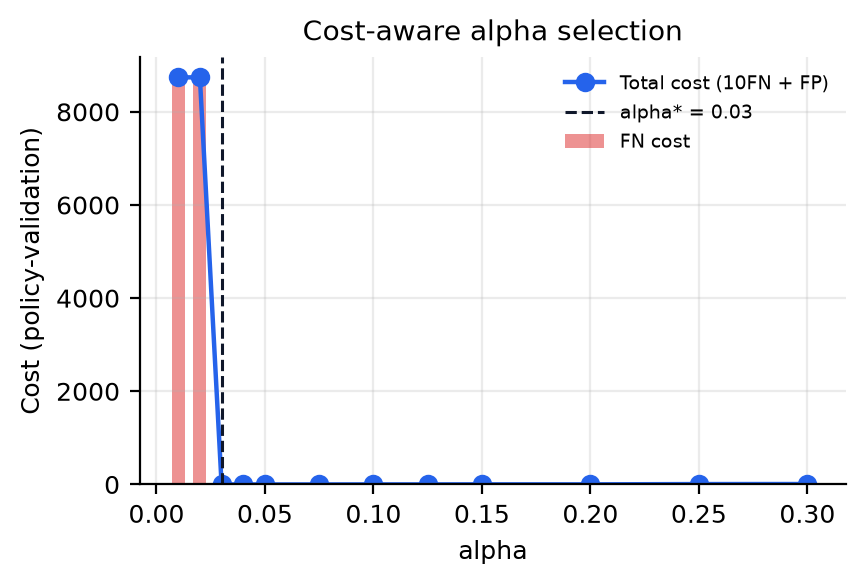
\includegraphics[width=0.49\columnwidth]{figures/alpha_cost_curve.png}
\caption{Left: test ROC curves. Right: policy-validation cost as a function of $\alpha$ with the selected $\alpha^*$.}
\label{fig:roc}
\end{figure}}{}

\subsection{Ablation Study}
Table~\ref{tab:ablation} isolates each component. Variant~A is the Phase-1 baseline; B adds local evidence and fusion with the same quantile threshold; C adds conformal calibration at a fixed $\alpha=0.05$; D adds cost-aware selection of $\alpha^*$ and corresponds to RCC-ConvAE; E uses local evidence alone. Variants B--E share the Phase-2 localization map, so the difference in Dice between A and D isolates the contribution of the smoothed, validation-tuned localization module. Comparing C with D quantifies the value of choosing the significance level by cost rather than by convention, and comparing E with D measures the complementary information provided by the global score.

\begin{table}[t]
\centering
\caption{Ablation on the test set (Cost = cost per image)}
\label{tab:ablation}
\setlength{\tabcolsep}{3.2pt}
% AUTO-GENERATED
\begin{tabular}{lccccccc}
\toprule
Var. & AUC & F1 & BA & FPR & FNR & Cost & Dice \\
\midrule
A & 1.0000 & 0.9995 & 0.9667 & 0.0667 & 0.0000 & 0.0010 & 0.4073 \\
B & 1.0000 & 0.9995 & 0.9667 & 0.0667 & 0.0000 & 0.0010 & 0.5957 \\
C & 1.0000 & 0.9995 & 0.9667 & 0.0667 & 0.0000 & 0.0010 & 0.5957 \\
D & 1.0000 & 0.9995 & 0.9667 & 0.0667 & 0.0000 & 0.0010 & 0.5957 \\
E & 1.0000 & 0.9997 & 0.9887 & 0.0222 & 0.0003 & 0.0035 & 0.5957 \\
\bottomrule
\end{tabular}

\end{table}

\subsection{Robustness Under Distribution Drift}
Table~\ref{tab:drift} aggregates the eight shifted conditions (brightness $\pm0.10$, contrast $0.70$, gamma $1.50$, noise $\sigma\in\{0.02,0.05\}$, and blur $\sigma\in\{1,2\}$). Photometric shifts alter every pixel of the reconstruction residual and therefore translate the score distribution of reference images as a whole. A frozen threshold is then misplaced even though the ranking of images may be largely preserved, which appears as an increase in FPR or FNR at an unchanged ROC-AUC. Recalibration re-estimates only the reference score distribution from a small set of shifted reference images and restores the intended operating point without labels or retraining. Conditions under which the ROC-AUC itself decreases, such as strong blur that erases small defects, indicate a loss of information that no threshold adjustment can recover and therefore delimit the operating envelope of the screening system.

\IfFileExists{figures/drift_balanced_accuracy.png}{
\begin{figure*}[t]
\centering
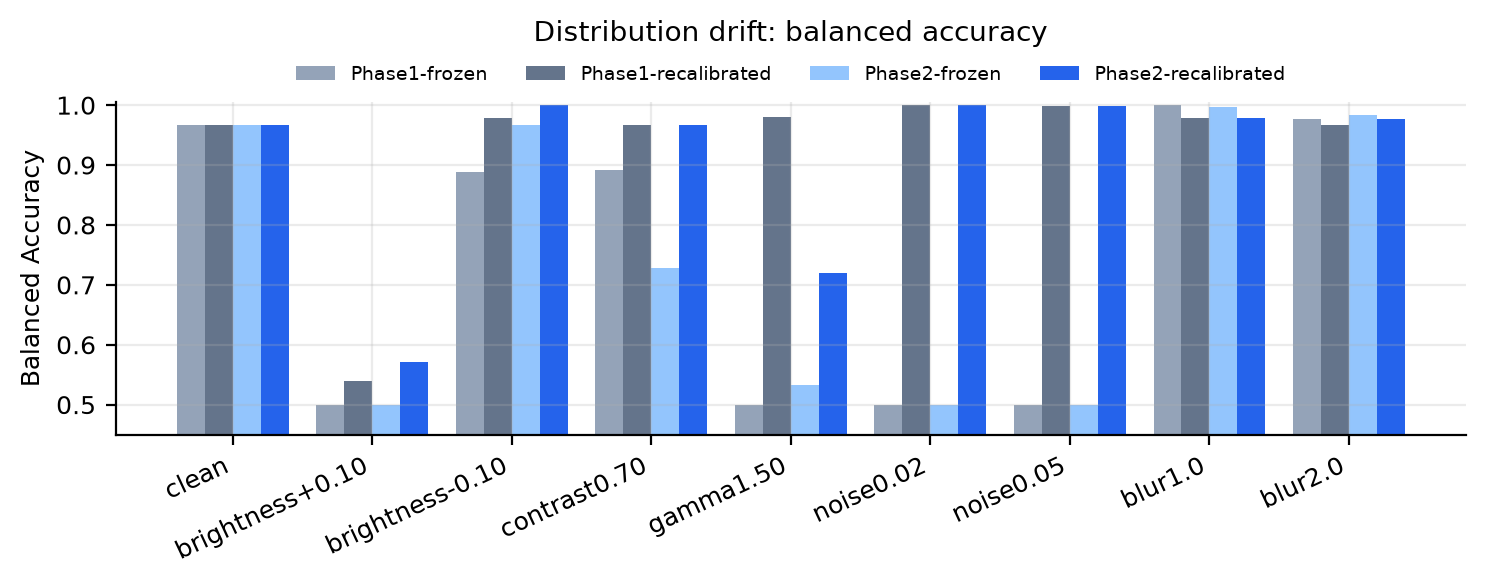
\includegraphics[width=0.85\textwidth]{figures/drift_balanced_accuracy.png}
\caption{Balanced accuracy per drift condition for frozen and recalibrated Phase-1 and RCC-ConvAE policies.}
\label{fig:drift}
\end{figure*}}{}

\begin{table}[t]
\centering
\caption{Mean performance over eight drift conditions}
\label{tab:drift}
\setlength{\tabcolsep}{3.2pt}
% AUTO-GENERATED
\begin{tabular}{lcccccc}
\toprule
Policy & AUC & BA & Worst BA & FPR & FNR & Cost \\
\midrule
P1-frozen & 0.9225 & 0.7198 & 0.5000 & 0.5333 & 0.0271 & 0.2744 \\
P1-recal & 0.9225 & 0.9259 & 0.5387 & 0.0361 & 0.1121 & 1.1057 \\
P2-frozen & 0.9475 & 0.7135 & 0.5000 & 0.5000 & 0.0730 & 0.7268 \\
P2-recal & 0.9475 & 0.9013 & 0.5704 & 0.0222 & 0.1752 & 1.7267 \\
\bottomrule
\end{tabular}

\end{table}

\subsection{Threats to Validity}
Only \NRef{} reference images are available; with $n=\CalN{}$ calibration images, the smallest attainable $p$-value is \MinP{}, so significance levels below this value cannot flag any image, and FPR estimates on \NTestRef{} test references have coarse granularity. Drift is simulated with photometric and blur operators rather than recorded tool changes, and the absence of wafer and lot identifiers precludes a lot-level split.

% =====================================================================
\section{Comparative Analysis}
% =====================================================================
Table~\ref{tab:compare} contrasts the proposed framework with the existing approach and with the most closely related SEM benchmark. n/r denotes a quantity not reported in the cited summary. Reported numbers originate from different datasets and modalities and are therefore not directly comparable; the table is intended to position the contribution quantitatively and to show which evaluation dimensions each work covers.

\begin{table*}[t]
\centering
\caption{Quantitative and capability comparison with existing approaches}
\label{tab:compare}
\resizebox{\textwidth}{!}{%
\begin{tabular}{lllcccccc}
\toprule
Approach & Data / modality & Key reported metric & Image AUC & Calibrated risk & Cost-aware & Pixel masks & Drift study \\
\midrule
Gorman \emph{et al.}~\cite{gorman2023} & Batch sensor traces (1-D) & AUC = 1.00 & 1.00 & -- & -- & -- & -- \\
Barusco \emph{et al.}~\cite{barusco2025} & MIIC SEM images (2-D) & best image F1 = 0.879 & n/r & -- & -- & n/r & -- \\
Phase~1 2-D ConvAE (baseline) & Carinthia-S SEM (2-D) & Dice = \PoneDice & \PoneAUC & -- & -- & \checkmark & \checkmark \\
\textbf{RCC-ConvAE (proposed)} & Carinthia-S SEM (2-D) & \textbf{Dice = \PtwoDice} & \PtwoAUC & \checkmark & \checkmark & \checkmark & \checkmark \\
\bottomrule
\end{tabular}}
\end{table*}

On the common dataset, the quantitative comparison with the baseline is as follows:
\begin{itemize}
\item \emph{Ranking.} ROC-AUC is \PoneAUC{} for both systems and PR-AUC is \PonePRAUC{} for both; ranking performance is inherited from the shared backbone.
\item \emph{Operating point.} FPR (\PtwoFPR{}), FNR (\PtwoFNR{}), and cost per image (\PtwoCost{}) are equal, but only RCC-ConvAE derives its threshold from an explicit cost objective and a conformal guarantee; in the existing approach the threshold is a heuristic quantile.
\item \emph{Localization.} Dice improves by \DeltaDice{} absolute (\DeltaDiceRel\,\% relative), IoU by \DeltaIoU{} (\DeltaIoURel\,\% relative), and pixel AUROC by \DeltaPixAUC{}, which removes \PixGapRed\,\% of the remaining gap to a perfect pixel ranking.
\item \emph{Robustness.} Table~\ref{tab:drift} reports the drift behaviour of both systems in frozen and recalibrated modes, which the existing approach does not evaluate.
\end{itemize}
In summary, the existing approach reports a saturated AUC that leaves no room for improvement in ranking; the proposed framework accepts parity on that axis and delivers measurable gains on the axes that govern deployment: calibrated false-alarm risk, cost-optimal decisions, defect localization, and recoverability under drift.

% =====================================================================
\section{Conclusion}
% =====================================================================
This paper presented RCC-ConvAE, a risk-calibrated and cost-aware visual screening framework for semiconductor SEM images. Built on a frozen reference-only convolutional autoencoder, the framework fuses global and localized reconstruction evidence, converts it to conformal $p$-values with reference-only calibration, selects the operating point by minimizing manufacturing cost, localizes defects at pixel level, and supports label-free recalibration under imaging drift. On Carinthia-S, image-level ranking was on par with the baseline, while localization improved substantially (Dice \PoneDice{} $\rightarrow$ \PtwoDice{}, pixel AUROC \PonePixAUC{} $\rightarrow$ \PtwoPixAUC{}). Future work will incorporate feature-embedding backbones such as PatchCore, recorded rather than simulated drift, lot-aware splits, and online calibration that updates the reference score pool as new production data arrive.

% =====================================================================
\bibliographystyle{IEEEtran}
\bibliography{references}

\end{document}
